\documentclass[11pt]{cornouaille}

\newrgbcolor{Rfond}{.995 0.945 .985}
\newrgbcolor{Rougef}{.8 0.1 .2}
\newrgbcolor{Rbord}{.6 0.1 .4}


\newcommand{\cadreR}[1]{%
\psframebox[framesep=.8em,linecolor=black,linewidth=0.25pt,framearc=0.2,fillstyle=solid,fillcolor=Rfond]{\begin{minipage}{\linewidth-1.6em}%
#1\end{minipage}}}

\usepackage{verbatim}


\begin{document}


\fexo{Spécialité première}{Chapitre 10 Les variables aléatoires}{Cours}

\section{Activité}



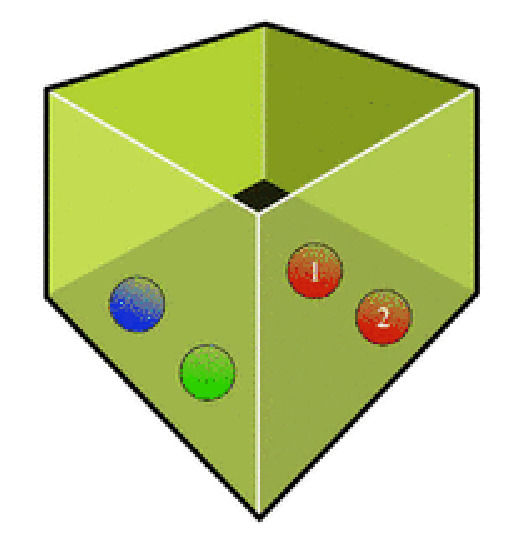
\includegraphics{./1S-VA-cours-0}


Une urne comprend une boule verte (V), une boule bleue (B) et deux
boules\\ rouges (R$_{1}$ et R$_{2}$).

On tire au hasard une boule, puis une deuxi\`{e}me sans avoir remis la
premi\`{e}re.




1.  Recopier et compl\'{e}ter l'arbre ci-contre afin de
d\'{e}terminer toutes\\ les issues possibles.



2.   Quelle est la probabilit\'{e} de chaque issue ?


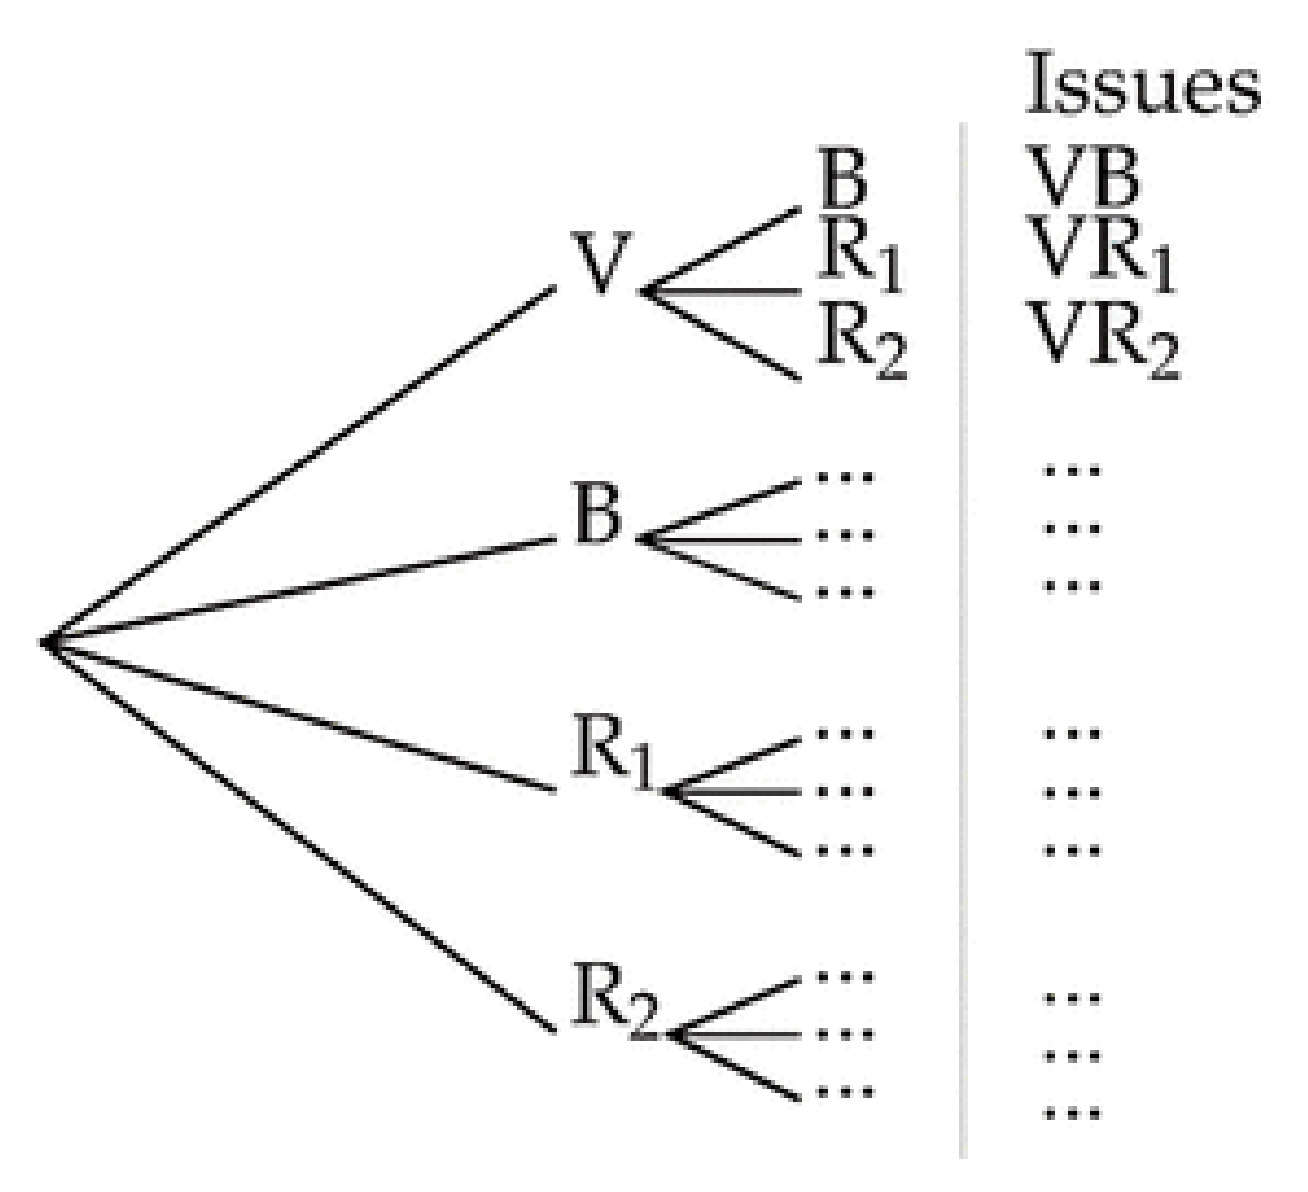
\includegraphics{./1S-VA-cours-1}



\vspace{-\baselineskip}



3.   Une boule bleue ne rapporte rien et ne fait rien perdre, une boule verte\\
rapporte 2 points et chaque boule rouge fait perdre 1 point.

On s'int\'{e}resse au gain alg\'{e}brique $X$ (positif ou
n\'{e}gatif) que peut obtenir\\ un joueur \`{a} ce jeu.




3. a)  Quelles sont les valeurs possibles pour le gain ?




3. b)  Recopier et compl\'{e}ter le tableau.




\begin{tabular}{|c|c|c|c|c|}
\hline
{\cellcolor{FondTableaux}\'{E}v\'{e}nement} & $\left( {X = - 2}
\right)$ & $\left( {X = - 1} \right)$ & $\left( {X = 1}
\right)$ & $\left( {X = 2} \right)$ \\\hline
{\cellcolor{FondTableaux} Issues favorables} & & & & \\\hline
\end{tabular}





3. c)   Calculer la probabilit\'{e}, not\'{e}e $P\left( {X
= - 2} \right)$, que le joueur perde 2 euros.



3. d)  Calculer de m\^{e}me $P\left( {X = - 1} \right)$, $P\left(
{X = 1} \right)$ et $P\left( {X = 2} \right)$.






\textbf{Correction}



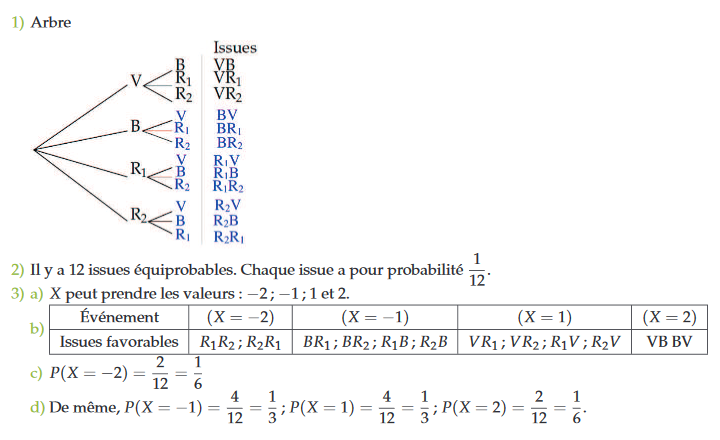
\includegraphics[scale=0.8]{corr1.png}


\bigskip

{\color{red}

COMMENTAIRES  :


$X$ s'appelle une variable aléatoire : "variable" car elle prend des valeurs numériques qui varient et "aléatoire" car ces valeurs prises dépendent du hasard.

Dans une expérience aléatoire, on cherche d'abord à l'aide de l'énoncé TOUTES les valeurs possibles que peut prendre $X$.

On veut ensuite trouver avec quelle probabilité chacune de ces valeurs peut être obtenue : on appelle cela le tableau de loi de la variable aléatoire $X$.

Une fois connu le tableau de loi on peut répondre à n'importe quelle question sur cette expérience et pourquoi pas, parier en toute connaissance de cause.

Dans ce cours, on va formaliser tout ceci :

}
\section{Notion de variable aléatoire réelle}

\cadreR{


Variable aléatoire discr\`{e}te

Soit $\Omega = \left\{ {{e_1};{e_2};...;{e_m}} \right\}$ l'univers
fini d'une exp\'{e}rience al\'{e}atoire.

Une \textbf{variable aléatoire}{} $X$ sur $\Omega$ est une
fonction qui, \`{a} chaque issue de $\Omega$, associe un nombre
r\'{e}el.
}

\bigskip

\bigskip

\textbf{Remarque}

\bigskip
$x$ est un r\'{e}el, l'\'{e}v\'{e}nement "$X$ prend la valeur $x$"
est not\'{e} ($X = x$), il est form\'{e} de toutes les issues de
$\Omega$ ayant pour image $x$.

\bigskip

\bigskip

\textbf{Application et méthode :}

\bigskip

\textbf{Enoncé:}
On lance un dé à 6 faces.

Si on obtient un multiple de 3, on gagne 2 euros.

Sinon, on perd 1 euro.

$X$ est la variable aléatoire qui à chaque lancer associe le gain obtenu (ce gain peut éventuellement être négatif)

\bigskip

\textbf{Méthode}

\bigskip

On cherche toutes valeurs possibles prises par la variable aléatoire $X$.

On écrit : $X$ désigne .........

puis : $X$ prend les valeurs ................

\bigskip

{\color{red}\textbf{Solution}

$X$ désigne le gain obtenu à un lancer

$X$ prend les valeurs 1 ou 2

L'évènement $(X=2)$ est réalisé lorsque l'on obtient un multiple de 3

L'évènement $(X \leq 0)$ est réalisé lorsque le gain est négatif


}
\bigskip

\newpage

\section{Loi de probabilité d'une variable aléatoire réelle}


\cadreR{


Loi de probabilit\'{e} d'une variable
al\'{e}atoire discr\`{e}te


Soit $X$ une variable al\'{e}atoire prenant les valeurs $\left\{
{x_1};{x_2};...;{x_n} \right\}$. Lorsqu'\`{a} chaque valeur
${x_i}$, on associe la probabilit\'{e} de l'\'{e}v\'{e}nement ($X =
x_{i}$) , on d\'{e}finit \textbf{la loi de probabilit\'{e}} de $X$.
}

\bigskip

\textbf{Remarque}

La loi de probabilit\'{e} d'une variable al\'{e}atoire se
pr\'{e}sente \`{a} l'aide d'un tableau.




\begin{tabular}{|*5{c|}}
\hline
\cellcolor{FondTableaux}${x_i}$                       & ${x_1}$ & ${x_2}$ & \ldots{} & ${x_n}$ \\\hline
\cellcolor{FondTableaux}$P\left( {X = {x_i}} \right)$ & ${p_1}$ & ${p_2}$ & \ldots{} & ${p_n}$ \\\hline
\end{tabular}


On a $P\left( {X = {x_1}} \right) + P\left( {X = {x_2}} \right) +
... + P\left( {X = {x_n}} \right) = 1$.

\bigskip

\bigskip

\textbf{METHODE A TRAVAILLER} \danger

\bigskip


\'{E}tudier une variable al\'{e}atoire :

\bigskip

\cadreR{
Pour d\'{e}terminer la loi de probabilit\'{e} d'une variable
al\'{e}atoire $X$ :




1.  on d\'{e}termine les valeurs ${x_i}$ que peut
prendre $X$ ;



2.  on calcule les probabilit\'{e}s $P\left( {X = {x_i}}
\right)$ ;



3.  on r\'{e}sume les r\'{e}sultats dans un tableau.


}

\bigskip

\bigskip


:::exercice Exercice 1:


Une urne contient cinq jetons indiscernables au toucher
num\'{e}rot\'{e}s de 1 \`{a} 5.

Un joueur participe \`{a} la loterie en payant 2~\euro, ce qui lui
donne le droit de pr\'{e}lever au hasard un jeton dans l'urne.

\begin{itemize}
\item Si le num\'{e}ro est pair, il gagne en euros le
double de la valeur indiqu\'{e}e par le jeton.

\item Si le num\'{e}ro est impair, il perd sa mise.
\end{itemize}


Soit $X$ la variable al\'{e}atoire \'{e}gale au "gain
alg\'{e}brique".

D\'{e}terminer la loi de probabilit\'{e} de $X$.



:::




\bigskip

{\color{red}

CORRECTION :


L'univers est l'ensemble des 5 jetons.

Les cinq issues sont \'{e}quiprobables.

Les jetons 1, 3~et 5 font perdre 2 euros ;

le jeton 2 fait gagner $2 \times 2 - 2 = 2$ euros ;

le jeton 4 fait gagner $4 \times 2 - 2 = 6$ euros.

$X$ peut prendre les valeurs $ - 2$ ; 2~et 6.

L'\'{e}v\'{e}nement $\left( {X = - 2} \right)$ est r\'{e}alis\'{e}
pour les issues 1 ; 3 ; 5 donc $P\left( {X = - 2} \right) =
\dfrac{3}{5}$.

L'\'{e}v\'{e}nement $\left( {X = 2} \right)$ est r\'{e}alis\'{e}
pour l'issue 2 donc $P\left( {X = 2} \right) = \dfrac{1}{5}$.

L'\'{e}v\'{e}nement $\left( {X = 6} \right)$ est r\'{e}alis\'{e}
pour l'issue 4 donc $P\left( {X = 6} \right) = \dfrac{1}{5}$.

On pr\'{e}sente la \textbf{loi de probabilit\'{e}} de $X$ dans un
tableau.




\begin{tabular}{|*4{c|}}
\hline
\cellcolor{FondTableaux}
${x_i}$                       & $ - 2$        & 2             & 6             \\      \hline
\cellcolor{FondTableaux}
$P\left( {X = {x_i}} \right)$ & $\dfrac{3}{5}$ & $\dfrac{1}{5}$ & $\dfrac{1}{5}$ \\      \hline
\end{tabular}


}




\section{Espérance, variance et écart-type}

Dans cette partie, $X$ est une variable aléatoire réelle définie sur un univers $\Omega$ prenant les valeurs $x_1$​, $x_2$​, ..., $x_r$​ avec les probabilités respectives $p_1$​, $p_2$​, ..., $p_r$​.

\bigskip

\subsection{Espérance d'une variable aléatoire}

\cadreR{
L'espérance de $X$ est le nombre réel, noté $E(X)$, défini par
$E(X)=\sum ​p_i​x_i​=p_1​x_1​+p_2​x_2​+…+p_r​x_r$​
}

\bigskip

\textbf{Remarque:}

$E(X)$ peut s'interpréter comme la valeur moyenne des valeurs prises par $X$ lorsque l'expérience aléatoire est répétée un très grand nombre de fois.

\bigskip

\textbf{Exemple:}

La loi de probabilité d'une variable aléatoire $X$ est donnée ci-dessous :


\begin{tabular}{|c|c|c|c|}
\hline
$x_i$​ &	$-2$ &	1 &	4 \\
\hline
$P(X=x_i​) $ &	$\frac{1}{6}$​ &	$\frac{1}{2}$​ &	$\frac{1}{3}​$ \\
\hline
\end{tabular}



On a $E(X)=−2 \times \frac{1}{6}​+1 \times \frac{1}{2}​+4 \times \frac{1}{3}​=\frac{3}{2}​$.

Sur un très grand nombre d'expériences, en moyenne, la valeur de $X$ est $\frac{3}{2}$​.

\bigskip

\textbf{Remarque:}

\cadreR{
Dans un jeu de hasard, l'espérance sera liée au gain potentiel du joueur (ou de l’organisateur).

\begin{itemize}
\item Un jeu est équitable si l'espérance du gain est nulle.
\item Un jeu est favorable au joueur si l'espérance est positive
\item Un jeu est défavorable au joueur si l'espérance est négative
\end{itemize}

}

\bigskip

\cadreR{


Propriété

Soit $X$ une variable aléatoire et soient $a$ et $b$ des réels. Alors : $E(aX+b)=a \times E(X)+b$.
}

\bigskip

\emph{Démonstration à faire plus tard}

\bigskip

\textbf{METHODE}


:::exercice Exercice 2:



Soit X une variable aléatoire dont on donne la loi de probabilité dans le tableau suivant. Calculer et interpréter $E(X)$.


\begin{tabular}{|c|c|c|c|}
\hline
$x_i$​ &	$-2$ &	1 &	4 \\
\hline
$P(X=x_i​)$ &	$0,2$ &	$0,5$ &	$0,3$ \\
\hline
\end{tabular}





:::




\textbf{Méthode}




1.   On applique la formule du cours en remplaçant les $x_i​$ par les valeurs prises par la variable aléatoire $X$ et les $p_i$​ par les probabilités correspondantes.



2.  On interprète le résultat à l'aide d'une moyenne en se rappelant que cela est valable uniquement pour un très grand nombre d'expériences identiques réalisées.


\bigskip

{\color{red}\textbf{Correction:}

$E(X)=−2 \times 0,2+1 \times 0,5+4 \times 0,3=1,3$

Sur un très grand nombre de répétitions de cette expérience aléatoire, la valeur moyenne de $X$ est $1,3$.

}

\subsection{Variance et écart-type d'une variable aléatoire}

\cadreR{
La \textbf{variance de $X$} est le réel positif, noté $Var(X)$, défini par
$Var(X)​=\sum ​p_i​(x_i​-E(X))^2=p_1​(x_1​-E(X))^2+p_2​(x_2​-E(X))^2+…+p_r​(x_r​-E(X))^2$.​

\bigskip

L'\textbf{écart-type de $X$} est le nombre positif, noté $\sigma(X)$, défini par $\sigma(X)=Var(X)$
​.
}

\bigskip

\textbf{Remarque:}


L'écart-type de $X$ est la moyenne quadratique des écarts des valeurs avec l’espérance.

\bigskip

\bigskip

\textbf{Exemple:}

On reprend la variable aléatoire $X$ de l'exemple précédent.

On a:

$Var(X)​=\frac{1}{6} \times (-2-\frac{3}{2}​)^2+\frac{1}{2}​ \times (1-\frac{3}{2}​)^2+\frac{1}{3} \times (4-\frac{3}{2}​)^2=\frac{1}{6}​ \times (-\frac{7}{2})^2+\frac{1}{2}​ \times (−\frac{1}{2})^2+\frac{1}{3} \times (2\frac{5}{2})^2=\frac{1}{6} \times \frac{49}{4}​+\frac{1}{2} \times \frac{1}{4}+\frac{1}{3} \times \frac{25}{4}​=\frac{17}{4}$

et

$ \sigma(X)=\sqrt{Var(X)}=\sqrt{\frac{17}{4}}=\frac{\sqrt{17}}{2}$
​

​​\textbf{Exemple:}


:::exercice Exercice 3:



Soit $X$ une variable aléatoire dont on donne la loi de probabilité dans le tableau suivant. Calculer la variance et l'écart-type de la variable aléatoire $X$.

\begin{tabular}{|c|c|c|c|}
\hline
$x_i$​ &	$-2$ &	1 &	4 \\
\hline
$P(X=x_i​)$ &	$0,2$ &	$0,5$ &	$0,3$ \\
\hline
\end{tabular}




:::




\bigskip

\textbf{Méthode:}


\begin{itemize}
\item On applique la formule du cours en remplaçant les $x_i$​ par les valeurs prises par la variable aléatoire $X$ et les $p_i$​ par les probabilités correspondantes.
\item L'écart-type s'obtient simplement en calculant la racine carrée de la variance
\end{itemize}


\bigskip

{\color{red}

\textbf{Correction:}

On a vu précédemment que $E(X)=1,3$.

On a alors :

$Var(X)​=0,2 \times (−2−1,3)^2+0,5 \times (1−1,3)^2+0,3 \times (4−1,3)^2=0,2 \times (−3,3)^2+0,5 \times 0,32+0,3 \times 2,72=0,2 \times 10,89+0,5 \times 0,09+0,3 \times 7,29=2,178+0,045+2,187=4,41​$

D’où $\sigma(X)=\sqrt{Var(X)}=\sqrt{4,41}=2,1$

}

\newpage

\section{Simulation d'une variable aléatoire}

Un jeu consiste à lancer $n$ fois deux dés parfaitement équilibrés.

Lorsqu'on obtient un double, on gagne 5 euros, sinon on perd 1 euro.

\bigskip


\begin{verbatim}

from random import randint
n=int(input("Quel est le nombre de lancers?"))
G=0
for i in range(n):
R=randint(1,6)
S=randint(1,6)
if R==S:
G=G+5
else:
G=G-1
print(G/n)
\end{verbatim}


\bigskip





1.  On consid\`{e}re l'algorithme ci-dessus.




1. a)  Qu'affiche cet algorithme ?



1. b)  Programmer cet algorithme sur une calculatrice ou un
logiciel.

Effectuer plusieurs simulations pour $n$ = 10 ; $n$ = 50 et $n$ =
100. Que constate-t-on ?




2.  Recopier et compl\'{e}ter le tableau \`{a} double entr\'{e}e.




\begin{tabular}{|*7{c|}}
\hline
\rowcolor{FondTableaux}
{\cellcolor{white}}
& 1  & 2    & 3 & 4 & 5 & 6 \\       \hline
\cellcolor{FondTableaux}1 & +5 & $-1$ &   &   &   &   \\    \hline
\cellcolor{FondTableaux}2 &    &      &   &   &   &   \\     \hline
\cellcolor{FondTableaux}3 &    &      &   &   &   &   \\       \hline
\cellcolor{FondTableaux}4 &    &      &   &   &   &   \\       \hline
\cellcolor{FondTableaux}5 &    &      &   &   &   &   \\       \hline
\cellcolor{FondTableaux}6 &    &      &   &   &   &   \\       \hline
\end{tabular}





3.   Calculer la probabilit\'{e} $p$ de perdre 1 euro, puis
la probabilit\'{e} $q$ de gagner 5 euros \`{a} ce jeu.



4.  Soit $X$ la variable aléatoire correspondant au gain de ce jeu.

\begin{itemize}
\item Quelles sont les valeurs prises par $X$ ?
\item Donner le tableau de loi de la variable aléatoire $X$ (vous pouvez vous aider de la question précédente)
\item Calculer l'espérance de $X$
\item Que pensez-vous du gain moyen que peut esp\'{e}rer le
joueur sur un grand nombre de parties ? Ce jeu favorise-t-il le
joueur ou l'organisateur ?
\end{itemize}






\bigskip

{\color{red}

\textbf{Correction:}



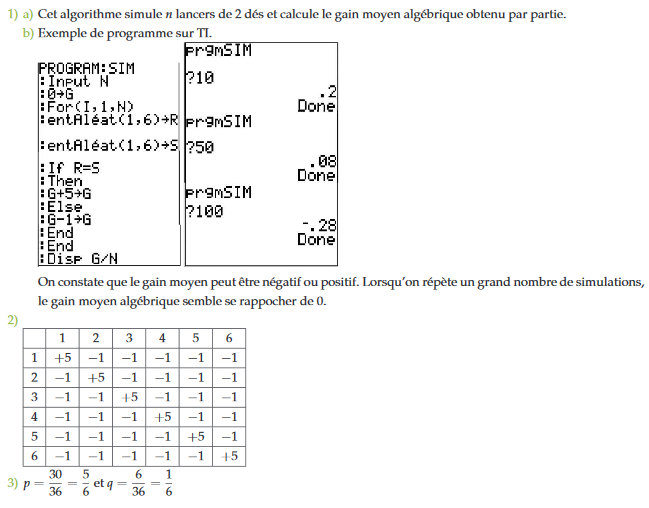
\includegraphics[scale=0.9]{algo1.png}


$X$ prend les valeurs $5$ ou $-1$.

$P(X=5)=\frac{cas favorables}{cas possibles}=\frac{6}{36}=\frac{1}{6}$

$P(X=-1)=\frac{cas favorables}{cas possibles}=\frac{30}{36}=\frac{5}{6}$


Loi de probabilité :




\begin{tabular}{|c|c|c|}
\hline
$x_i$ & 5 & $-1$ \\
\hline
$P(X=x_i)$ & $\frac{1}{6}$ & $\frac{5}{6}$ \\
\hline

\end{tabular}



Calcul de l'espérance :

$E(X)=5 \times \frac{1}{6}+(-1) \times \frac{5}{6}=0$

L'espérance est nulle, le jeu est donc équitable (le jeu ne favorise ni le joueur ni l'organisateur)
}
\end{document}